\chapter{Introducción}
Este Trabajo Fin de Grado se centra en el campo de las tecnologías Web. En este capitulo vamos a introducir los conceptos de básicos de la comunicación entre los navegadores y las aplicaciones web.Ademas se ofrece una visión general de aplicaciones que emplean tecnologías Web,que dan contexto a este TFG.
\section{Paradigma Cliente-Servidor}
La red (Internet) ofrece un servicio básico de comunicación (transferencia de bits). El software de comunicaciones (implementación de TCP/IP) de las máquinas no inicia comunicaciones con otras máquinas sino que son las aplicaciones.
Si nos centramos en el punto de vista funcional, se puede definir como una arquitectura distribuida que permite a los usuarios finales obtener acceso a información de forma transparente por medio de peticiones HTTP a un servidor, figura \ref{fig:Cliente_Servidor}.
\begin{figure}[!h]
\centering
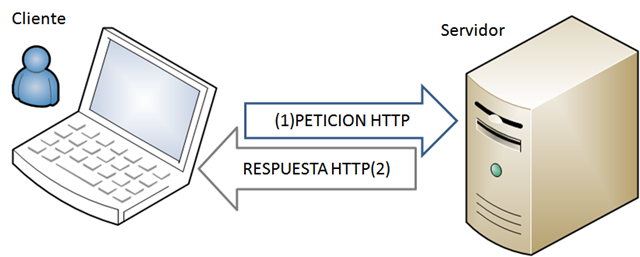
\includegraphics[width=0.5\linewidth]{Figures/Cliente_Servidor}
\decoRule
\caption[Esquema Cliente-Servidor]{Esquema Cliente-Servidor.}
\label{fig:Cliente_Servidor}
\end{figure}
\\La forma estándar de uso de sistemas Cliente/Servidor es a través de interfaces gráficas de usuario; mientras que la administración de datos y su seguridad e integridad se deja a cargo de los servidores.
\subsection*{Cliente}
Es el proceso que permite a los usuarios formular peticiones al servidor,a este proceso se le conoce como \textbf{front-end}.
\\Las principales funciones  que maneja son :
\begin{itemize}
\item Administrar la interfaz de usuario.
\item Interactuar con el usuario.
\item Procesar la lógica de la aplicación y hacer validaciones locales.
\item Generar requerimientos de bases de datos.
\item Recibir resultados del servidor.
\item Formatear resultados. 
\end{itemize}
\subsection*{Servidor}
Es el proceso encargado de atender a múltiples clientes que hacen peticiones de algún recurso administrado por él. A este se le conoce con el término \textbf{back-end }.
\\Las principales funciones  que maneja son:
\begin{itemize}
\item Aceptar los requerimientos de bases de datos que hacen los clientes.
\item Procesar requerimientos de bases de datos.
\item Formatear datos para trasmitirlos a los clientes.
\item Procesar la lógica de la aplicación y realizar validaciones a nivel de bases de datos.
\end{itemize}
\section{Tecnologías Web}
\subsection*{Protocolo HTTP}
Como se ha mencionado el modelo C/S se basa en peticiones entre cliente-servidor bajo el protocolo HTTP (\textbf{Hyper Text Transfer Protocol}).Este protocolo fue desarrollado por el \textit{World Wide Web Consortium}\footnote{Web: \url{http://www.w3.org/}} y la \textit{Internet Engineering Task Force}. 

Se compone de dos mensajes, el primer mensaje es originado por el cliente y es el requerimiento inicial de la comunicación. Este requerimiento llamado \textbf{Request} esta dividido en una cabecera y un mensaje de texto.En la cabecera el cliente envía información de la pagina solicitada al servidor y de la aplicación cliente que estamos utilizando en el \textbf{User-Agent},entre otras cosas.
\begin{lstlisting}[
caption=Peticion HTTP.]
 GET /index.html HTTP/1.1
 Host: www.example.com
 User-Agent: HTTPTool/1.0
 Connection: close
 Linea en blanco
\end{lstlisting}
Una vez recibido el requerimiento el servidor devuelve una respuesta llamada \textbf{Response} la cual también esta compuesta por una cabecera y un mensaje.
\begin{lstlisting}[
caption=Respuesta HTTP.]
 HTTP/1.1 200 OK
 Date: Fri, 31 Dec 2003 23:59:59 GMT
 Content-Type: text/html
 Content-Length: 1221
 <html><body>
 <h1>Pagina principal</h1>
 .. .
 </b d ></ht l>
\end{lstlisting}
Es un protocolo sin estado, es decir, que no guarda ninguna información sobre conexiones anteriores.
\subsection*{HTML}
Son las iniciales de la expresión en inglés HyperText Markup Language. Se trata de un conjunto de etiquetas que se van intercalando entre el texto de forma que los  navegadores sepan qué es lo que tienen que mostrar cuando accedemos a una página y cómo deben presentarlo en la pantalla.

El W3C (World Wide Web Consortium)\footnote{Web: \url{http://www.w3.org/}} es el fórum internacional que se encarga desarrollar nuevas tecnologías relacionadas con la WEB dictando las normas que constituyen el estándar HTML entre otros.A lo largo de sus diferentes versiones, se han incorporado y suprimido diversas características, con el fin de hacerlo más eficiente y facilitar el desarrollo de páginas web.
La versión mas extendida y estable fue 4.0 que permitía utilizar textos, sonidos, imágenes,y lo más importante, enlaces a otras páginas enriqueciendo de esta forma la información de la pagina.

Pero a medida que este lenguaje se extendía se vio la necesidad de actualizar la versión del estándar.Es aquí, donde surge la versión 5 \footnote{\url{http://www.w3.org/TR/2014/REC-html5-20141028/.}} de HTML que pretende cubrir varias necesidad que habían surgido hasta el momento. Dentro de estas nuevas características destacamos:
\begin{itemize}
\item \textbf{Contenido multimedia:} Habilita la posibilidad de incluir contenido multimedia de forma nativa sin necesidad de plugins o software de terceros.
\item \textbf{Animación:} Incluye la etiqueta canvas que permite crear contenido 2d y 3d dentro de la web.
\item \textbf{Comunicación:} con la aparición de aplicaciones en tiempo real, era necesario proveer de mecanismos que permitan intercambiar datos de forma ligera por lo que se incluye WebSockets y WeRTC.
\item \textbf{Animación:}PENDIENTE.
\end{itemize}
\section{Estado del arte}
Las fuentes\footnote{fuente:\url{http://www.revistadintel.es/Revista/Numeros/Numero16/Zona/Firmas/userosRedesSociales.pdf}} establecen tres generaciones de sitios Web.Actualmente conviven las distintas generaciones, aunque la creación de sitios web siguen el modelo de la segunda generación.
\subsection*{Primera generación}
Esta primera generación abarca desde el nacimiento de la Web(1992) hasta mediados de 1994 y es conocida como Web 1.0. 
\\Sus paginas eran simples documentos constituidos por texto e interpretadas por los navegadores existentes en ese momento.Algunos de los navegadores existentes eran Erwise(figura \ref{fig:Erwise5}(a)\footnote{fuente:\url{https://en.wikipedia.org/w/index.php?curid=24471738}}) y ViolaWWW(figura \ref{fig:Erwise5}(b)\footnote{fuente:  \url{https://en.wikipedia.org/w/index.php?curid=6098546}}
\begin{figure}[!h]
\centering
\subfigure[Navegador Erwise]{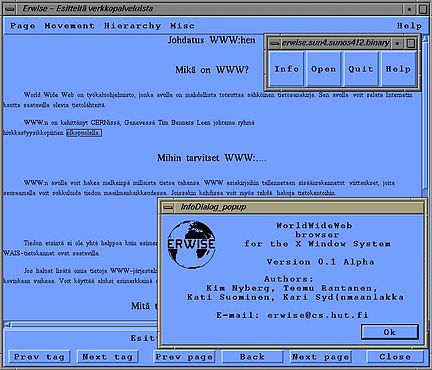
\includegraphics[width=50mm]{Figures/Erwise5}}
\subfigure[Navegador ViolaWWW]{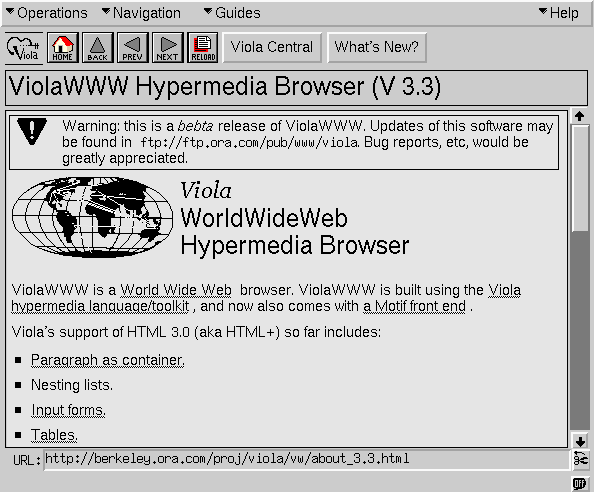
\includegraphics[width=50mm]{Figures/ViolaWWW}}
\caption{Navegadores de 1ª generación.} \label{fig:Erwise5}
\end{figure}
\\Posteriormente, con la aparición del lenguaje HTML, el concepto inicial de la Web 1.0 evoluciono convirtiéndose en un conjunto de documentos en lenguaje HTML que se encontraban interconectados por medio de enlaces.Estos documentos los generaba una única persona que se encargaba del diseño y de la obtención de los datos necesarios presentando como obstáculo que los documentos solo eran de lectura por lo que el usuario no tenia la capacidad de interactuar con el contenido de la pagina,figura \ref{fig:primera_Web}\footnote{fuente:\url{https://www.w3.org/History/19921103-hypertext/hypertext/WWW/TheProject.html}}.
\begin{figure}[!h]
\centering
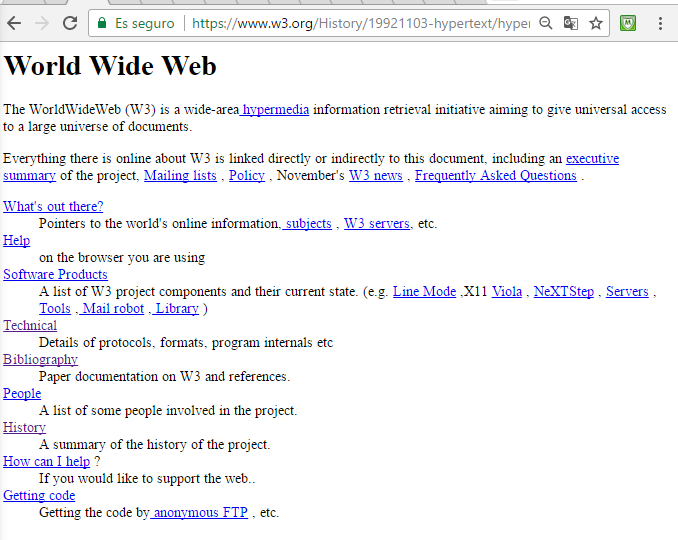
\includegraphics[width=0.4\linewidth]{Figures/primera_Web}
\decoRule
\caption[Ejemplo Web 1ª generación]{Ejemplo Web 1ª generación.}
\label{fig:primera_Web}
\end{figure}
\subsection*{Segunda generación}
Con la llegada de las “compañías cibernéticas” (año 2001) Internet da un giro de 180 grados. El éxito de estas compañías dependía  de webs mucho más dinámicas y para ello era necesario huir de sitios estáticos y poco actualizados, y servir páginas HTML dinámicas creadas al vuelo desde una actualizada base de datos. Los CMS (Content Management System o Sistema Gestor de Contenidos) entraron en acción.

Esta nueva generación recibe el nombre Web 2.0 .Este termino aparece por primera vez en el año 2004 cuando Dale Dougherty (vicepresidente de O’Reilly Media) utilizó este término en una conferencia en la que hablaba del renacimiento y evolución de la web.
\\Aunque no existe una definición consensuada, en el año 2005 Tim O’Reilly (fundador de O’Reilly Media) definió el concepto de Web 2.0 como “\textit{una serie de aplicaciones y páginas de Internet que utilizan la inteligencia colectiva para proporcionar servicios interactivos en red dando al usuario el control de sus datos}”.

A diferencia de la Web 1.0,la información y los contenidos se producen (directa o indirectamente) por los usuarios del sitio web y adicionalmente puede ser compartida por varios portales web de estas características.
\\Algunos ejemplos de la Web 2.0 son las las wikis(figura \ref{fig:wikipediaImagen}\footnote{fuente: \url{https://www.wikipedia.org/}}), los servicios multimedia (figura \ref{fig:youtubeImagen}\footnote{fuente:\url{https://www.youtube.com/}}) y en general sitios web que interactuan con los usuarios (figura \ref{fig:amazonImagen}\footnote{fuente:\url{https://www.amazon.es/}})
\begin{figure}[!h]
\centering
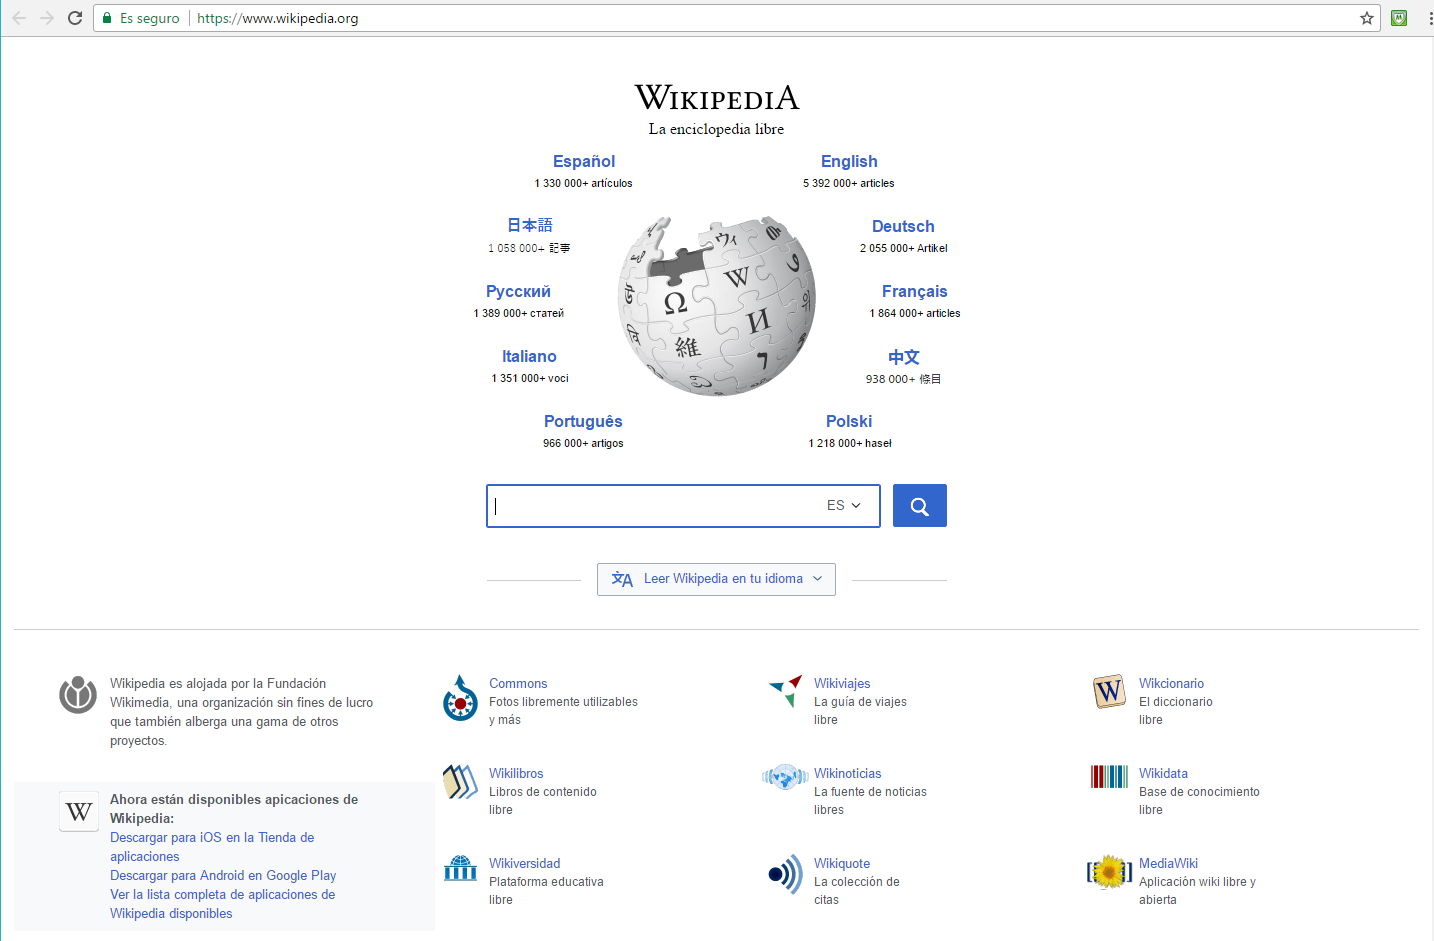
\includegraphics[width=0.5\linewidth]{Figures/wikipediaImagen}
\decoRule
\caption[Pagina Web:Wikipedia.]{Pagina Web:Wikipedia.}
\label{fig:wikipediaImagen}
\end{figure}
\begin{figure}[!h]
\centering
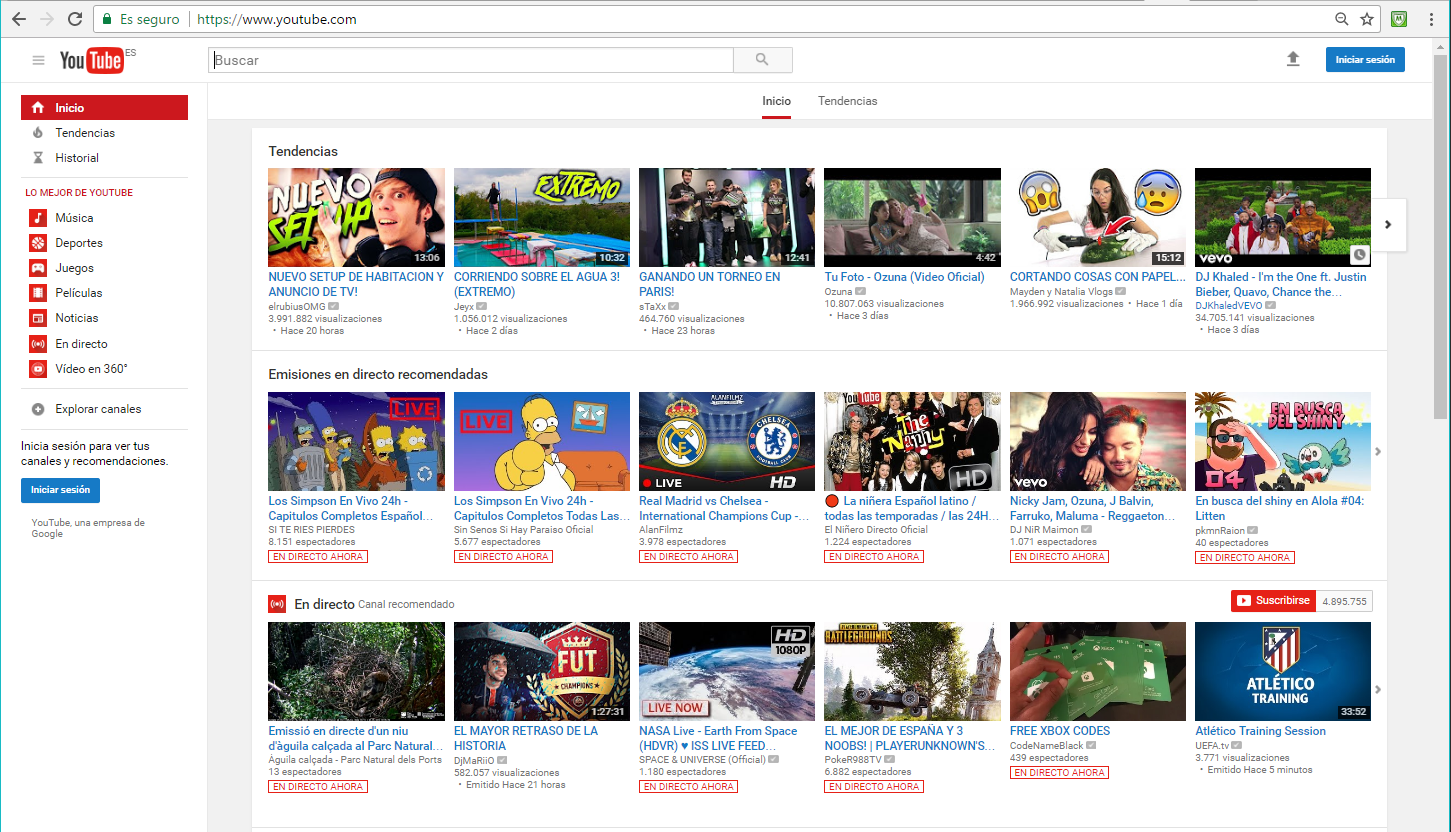
\includegraphics[width=0.5\linewidth]{Figures/youtubeImagen}
\decoRule
\caption[Pagina Web:YouTube.]{Pagina Web:YouTube.}
\label{fig:youtubeImagen}
\end{figure}
\begin{figure}[!h]
\centering
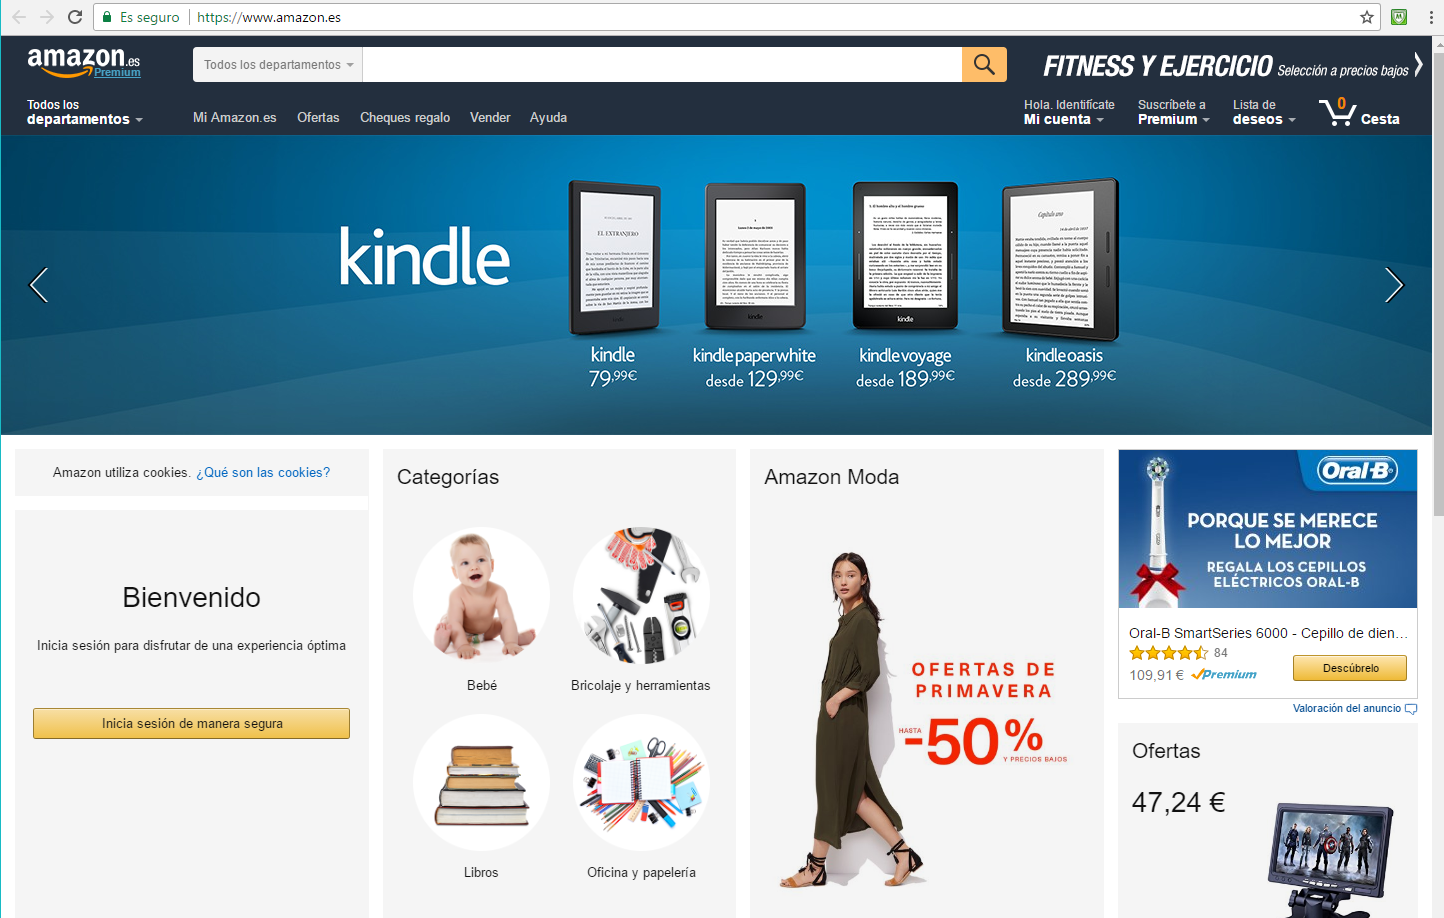
\includegraphics[width=0.5\linewidth]{Figures/amazonImagen}
\decoRule
\caption[Pagina Web:Amazon.]{Pagina Web:Amazon.}
\label{fig:amazonImagen}
\end{figure}
\\Al igual que la web evoluciona los navegadores\footnote{fuente:\url{http://www.mclibre.org/consultar/htmlcss/otros/otros\_historia\_navegadores.html\#navegadores}} también los hicieron.En la actualidad disponemos de los siguientes navegadores:
\begin{enumerate}
\item \textbf{Internet Explorer:} creado en 1995 aunque no fue hasta el año 2000 que domino absolutamente el mercado.Pero con la llegada de Firefox su uso global descendió de una forma notable.
\item \textbf{Firefox:} creado por la fundación Mozilla y es la continuación al navegador Mozilla.Se publico en 2004 con el objetivo de permitir que la web sea publica, abierta y accesible.
\item \textbf{Safari:} creado en 2003 para el sistema operativo Mac de Apple ya que antes no disponía de un navegador propio.
\item \textbf{Chrome:} creado en 2008 por Google a partir de WebKit.Destaca por su interfaz minimalista y por la velocidad de ejecución del código JavaScript,lo que obligo a sus competidores a ponerse las pilas en estos aspectos.
\end{enumerate}
A continuación se muestra una comparativa\footnote{fuente:\url{http://identidadgeek.com/por-que-el-navegador-opera-no-es-tan-popular/2011/01/}} del porcentaje de uso de cada uno de los navegadores en la actualidad.
\begin{figure}[!h]
\centering
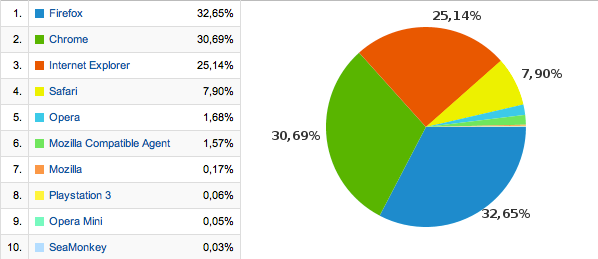
\includegraphics[width=0.4\linewidth]{Figures/uso_navegadores}
\decoRule
\caption[Comparativa del uso de los navegadores]{Comparativa del uso de los navegadores.}
\label{fig:uso_navegadores}
\end{figure}
\subsection*{Tercera generación}
En el intento de comprender la propia Web 2.0 se vislumbran futuras etapas de la Web, sobre todo orientadas a mejorar la interactividad y la movilidad entre/de los usuarios.
\\El término Web 3.0 está asociado al concepto de Web Semántica, desarrollado bajo la tutela del creador de la Web Tim Berners Lee. 
\\Básicamente, toda la información publicada en las diferentes páginas web no es entendible por los ordenadores, teniendo únicamente significado para las personas. La idea consiste en añadir información adicional a la información “visible”, de tal manera que pueda ser entendida por los ordenadores.
\\En conclusión, se trata de dotar de significado a las paginas web
\section{Antecedentes}
Como se ha mencionado a lo largo del capitulo las tecnologías web permiten crear interfaces para que los usuarios interactuan con las prestaciones de la aplicación. A continuación se muestra como ejemplo de esto dos TFG que incorporan tecnologías Web en su desarrollo ya sea para la creación de un interfaz como para intercambiar información entre el cliente y el servidor de la aplicación.
\subsection*{Surveillance 5.1 (URJC)}
Surveillance 5.1 \cite{TFGsurveillance5.1}\cite{surveillance5.1} fue desarrollado por Edgar Barrero como trabajo fin de grado.La aplicación web ofrece un flujo de vídeo desde una cámara web, un flujo de imagen de profundidad procedente de un sensor Kinect y su representación en 3D. También ofrece el acceso a un sensor de humedad y un actuador como ejemplos de dispositivos domoticos.
\\Su desarrollo se creo por medio de Ruby on Rails, un entorno de condigo abierto para el desarrollo de aplicaciones web. El servidor web se conecta a componentes JdeRobot que ofrecen interfaces ICE de objetos distribuidos. De esta forma obtiene datos de los distintos sensores y actuadores de la aplicación. En el lado cliente, el navegador refresca
estos datos realizando peticiones AJAX.
\begin{figure}[!h]
\centering
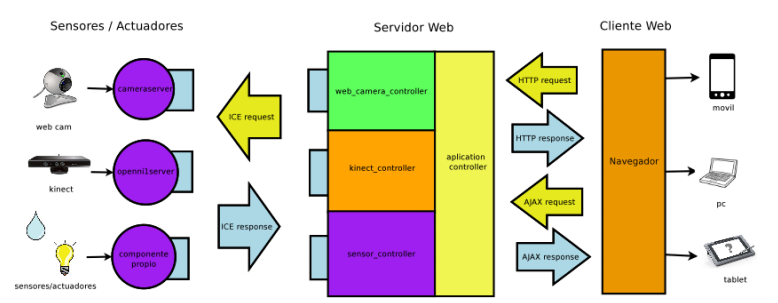
\includegraphics[width=0.5\linewidth]{Figures/edgar_surveillance_esquema}
\decoRule
\caption[Esquema Surveillance 5.1]{Esquema Surveillance 5.1.}
\label{fig:edgar_surveillance_esquema}
\end{figure}
\begin{figure}[!h]
\centering
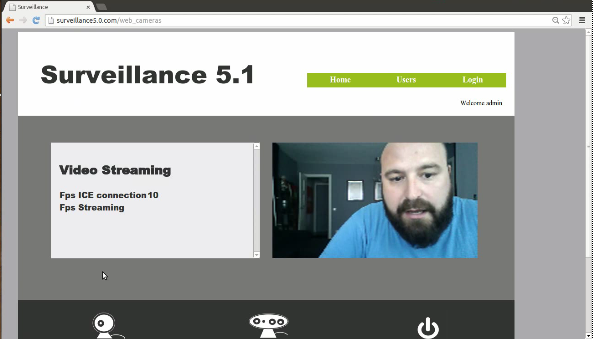
\includegraphics[width=0.5\linewidth]{Figures/edgar_surveillance5_web}
\decoRule
\caption[Interfaz Surveillance 5.1.]{Interfaz Surveillance 5.1.}
\label{fig:edgar_surveillance5_web}
\end{figure}
\subsection*{JdeRobotWebClients (URJC)}
JdeRobotWebClients\cite{TFGJdeRobotWebClients}\cite{JdeRobotWebClients}fue desarrollado por Aitor Martınez Fernandez como trabajo fin de grado.La aplicación Web ofrece la posibilidad de crear seis versiones web de herramientas utilizadas JdeRobot(CameraViewJS,RGBDViewerJS,KobukiViewerJS,.....) y que estaban programadas en C++ o Python con su propio interfaz gráfico provocando que sean ejecutables solo en Linux.Estas nuevas versiones pretenden ser multiplaforma (Linux, Android, IOS, Windows,...), y accesibles desde un navegador web como interfaz gráfico permitiendo acceder a los sensores y actuadores sin un servidor intermedio.
\begin{figure}[!h]
\centering
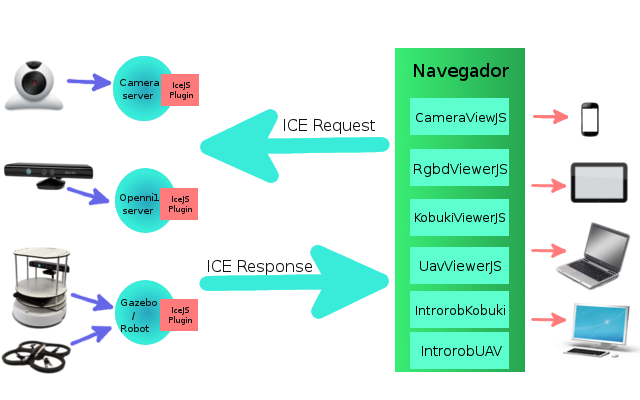
\includegraphics[width=0.5\linewidth]{Figures/Aitor_esq_proyecto}
\decoRule
\caption[Esquema JdeRobotWebClients]{Esquema JdeRobotWebClients.}
\label{fig:Aitor_esq_proyecto}
\end{figure}
\begin{figure}[!h]
\centering
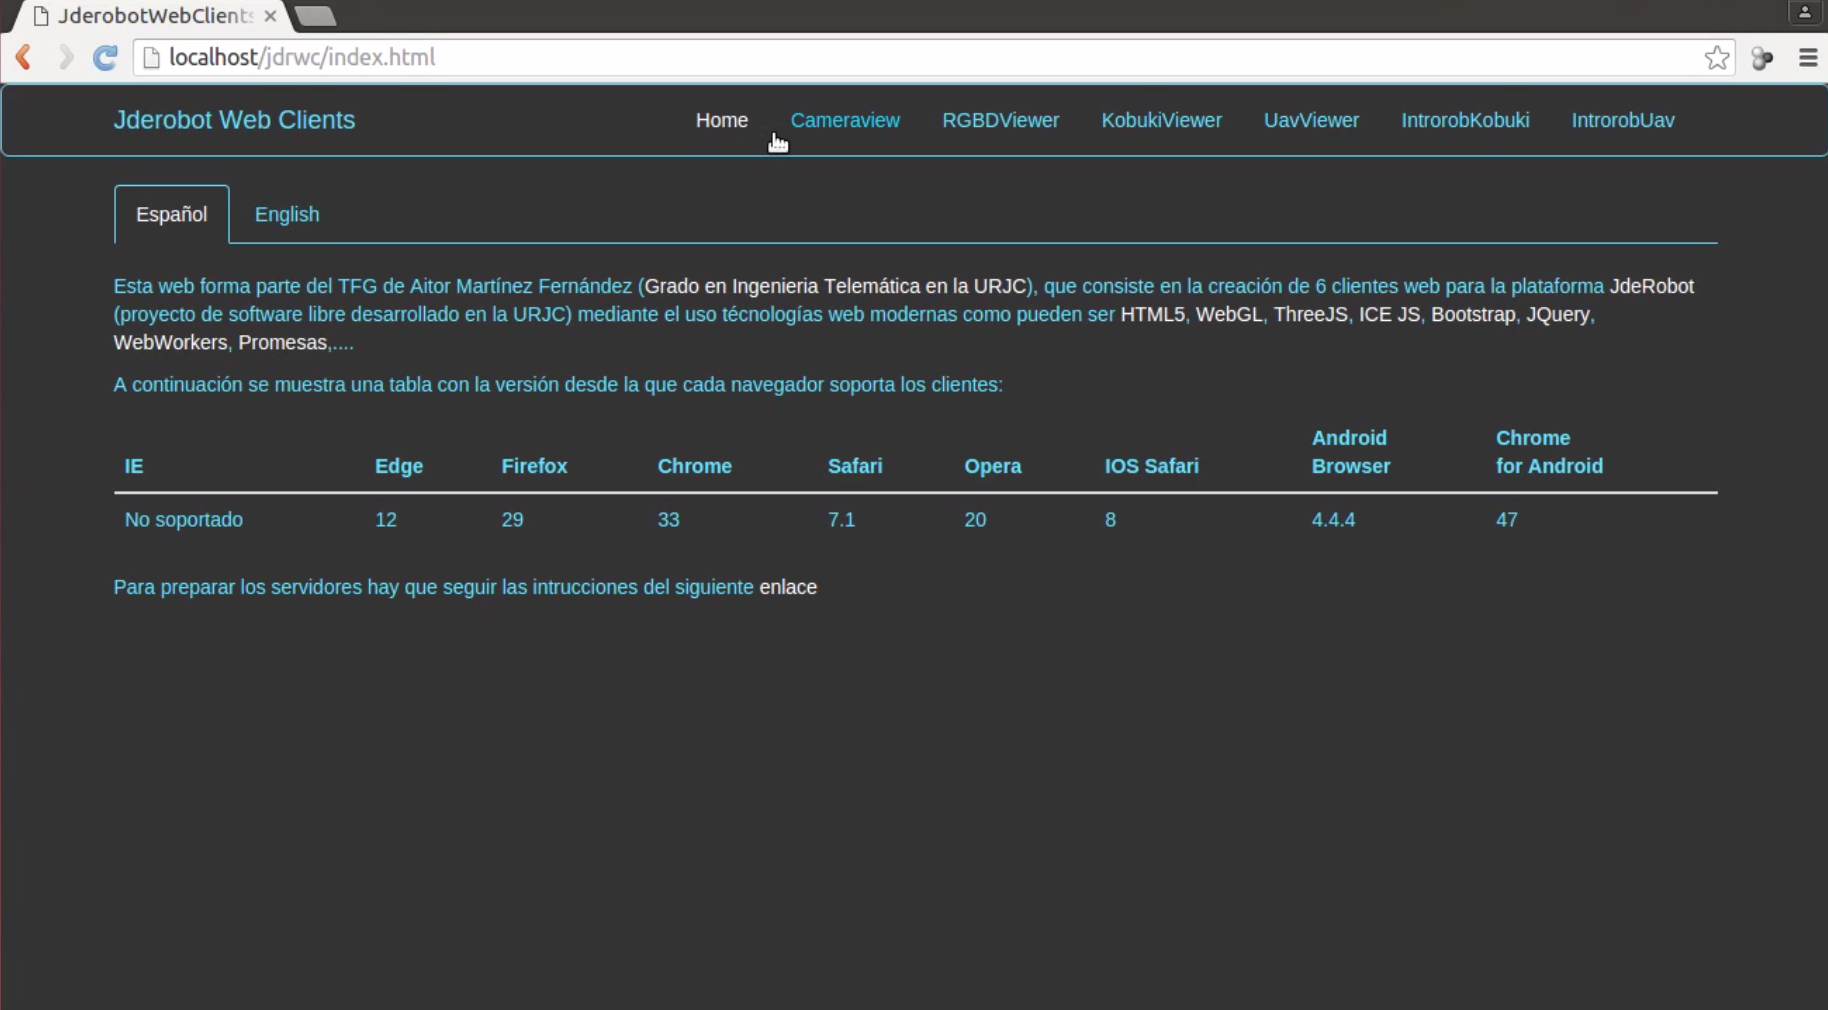
\includegraphics[width=0.5\linewidth]{Figures/Aitor_esquema_web}
\decoRule
\caption[Interfaz JdeRobotWebClients]{Interfaz JdeRobotWebClients.}
\label{fig:Aitor_esquema_web}
\end{figure}
